% Presentation Beamer file for course project review
\documentclass[11pt]{beamer}
\usetheme{Madrid}
\usepackage[utf8]{inputenc}
\usepackage[T1]{fontenc}
\usepackage{graphicx}
\usepackage{booktabs}
\usepackage{tikz}
\usetikzlibrary{calc,positioning,arrows.meta}
\usepackage{amsmath}
\title[Clean-Label Attacks on HAR]{Clean-Label Backdoor Attacks on Time-Series Human Activity Recognition}
\author[Nikhil, Chaitanya, Anasmit]{Nikhil \and Chaitanya \and Anasmit}
\institute[DS603 Project]{Departmental Project — DS603}
\date{November 2025}
\begin{document}

\begin{frame}
  \titlepage
\end{frame}

\begin{frame}{Outline}
  \begin{itemize}
    \item Motivation & Problem
    \item Key contributions
    \item Methodology (overview)
    \item Representative attack methods
    \item Selected results & takeaways
    \item Limitations, implications, next steps
  \end{itemize}
\end{frame}

\begin{frame}{Motivation}
  \begin{itemize}
    \item HAR systems are used in healthcare, wearables, and IoT — safety-critical domains.
    \item Clean-label poisoning: stealthy attacks that preserve true labels, evading simple checks.
    \item Question: Can explainability tools (LIME/SHAP) be used to guide effective, stealthy attacks on time-series models?
  \end{itemize}
\end{frame}

\begin{frame}{Key Contributions}
  \begin{itemize}
    \item Integrated LIME/SHAP analysis with feature-space and gradient-based poisoning for time-series HAR.
    \item Developed reproducible saliency-driven and explainability-guided attack pipelines for UCI-HAR and WISDM.
    \item Comprehensive evaluation across deep and traditional ML models; documented vulnerabilities and defenses needed.
  \end{itemize}
\end{frame}

\begin{frame}{Methodology — High Level}
  \centering
  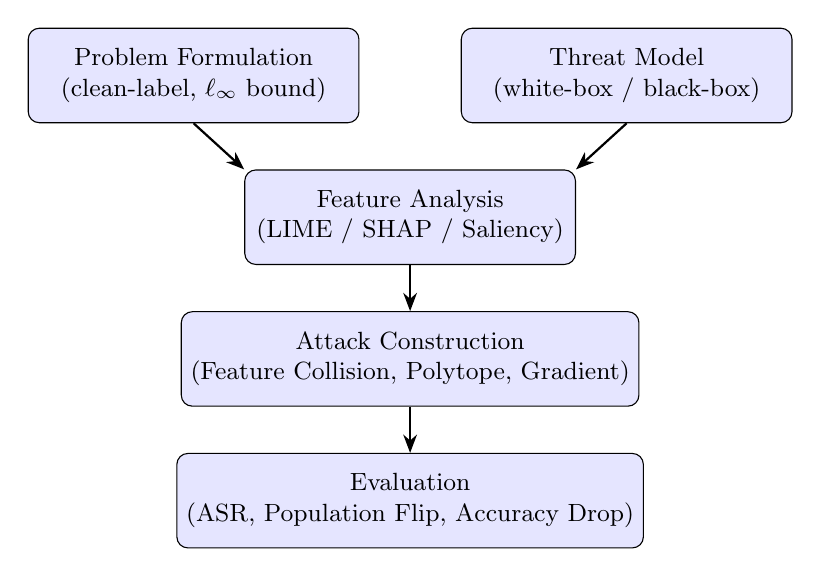
\begin{tikzpicture}[
      box/.style={rounded corners, draw, fill=blue!10, minimum width=42mm, minimum height=12mm, align=center, font=\small},
      arr/.style={-{Stealth}, thick}
    ]
    % Row 1: two boxes with explicit coordinates
    \node[box] (problem) at (0,0) {Problem Formulation\\(clean-label, $\ell_\infty$ bound)};
    \node[box] (threat)  at (5.5,0) {Threat Model\\(white-box / black-box)};

    % Row 2: centered below the pair
    \node[box] (analysis) at (2.75,-1.8) {Feature Analysis\\(LIME / SHAP / Saliency)};

    % Row 3 & 4
    \node[box] (attacks) at (2.75,-3.6) {Attack Construction\\(Feature Collision, Polytope, Gradient)};
    \node[box] (eval)    at (2.75,-5.4) {Evaluation\\(ASR, Population Flip, Accuracy Drop)};

    % Arrows
    \draw[arr] (problem.south) -- (analysis.north west);
    \draw[arr] (threat.south)  -- (analysis.north east);
    \draw[arr] (analysis) -- (attacks);
    \draw[arr] (attacks)  -- (eval);
  \end{tikzpicture}
\end{frame}

\begin{frame}{Representative Attack: Explainability-Guided}
  \begin{itemize}
    \item Use LIME/SHAP to compute channel/timestep importance matrix $W$.
    \item Optimize perturbations focusing on high-weight entries: feature collision, centroid shifts, polytope rings.
    \item Applicable in black-box scenarios (uses model-agnostic explainability or surrogate models).
  \end{itemize}
\end{frame}

\begin{frame}{Representative Attack: Saliency-Driven}
  \begin{itemize}
    \item Use gradient-based saliency to identify high-influence timesteps/channels.
    \item Construct deterministic target signature and blend into selected source-class windows.
    \item Enforce temporal continuity (50\% overlap) to keep samples plausible.
    \item Works well for identifying sensitive windows in CNNs.
  \end{itemize}
\end{frame}

\begin{frame}{Selected Results — Topline}
  \begin{itemize}
    \item WISDM (traditional ML vulnerability): Ridge classifier achieved \textbf{22.7\% ASR} with clean-label attacks.
    \item UCI-HAR (deep model robustness): CNN shows \textbf{< 4\% ASR} (1.2\% in our tests).
    \item Explainability: Y-acceleration emerged as a dominant feature on WISDM (\textasciitilde46\% importance by SHAP).
    \item Attacks preserve model utility: poisoned accuracy within 1--3\% of clean accuracy in most settings.
  \end{itemize}
\end{frame}

\begin{frame}{Implications \\ and Recommendations}
  \begin{itemize}
    \item Explainability tools can reveal attackable features — dual-use risk.
    \item Prefer robust architectures and preprocessing for safety-critical deployments.
    \item Defenses should include feature-space checks, temporal-consistency tests, and certified robustness where possible.
  \end{itemize}
\end{frame}

\begin{frame}{Limitations \& Future Work}
  \begin{itemize}
    \item Mostly single-target evaluations; multi-target and adaptive defenses remain to be explored.
    \item Need experiments on Transformer-based models and physical-sensor realizability.
    \item Next: implement defense baselines (spectral signatures, activation clustering) and cross-architecture transfer tests.
  \end{itemize}
\end{frame}

\begin{frame}{Appendix: Implementation Notes}
  \begin{itemize}
    \item Code: PyTorch-based; scripts enforce clean-label constraint (labels copied, only features modified).
    \item Perturbation bounds: $\ell_\infty$ (UCI-HAR: $\varepsilon=0.02$, WISDM: $\varepsilon=0.3$).
    \item Reproducibility: deterministic seeding and overlapping-window constraints used across experiments.
  \end{itemize}
\end{frame}

\begin{frame}{Thank you / Contact}
  \begin{itemize}
    \item Questions welcome — we can expand any slide.
    \item Authors: Nikhil, Chaitanya, Anasmit
    \item Project repo: (available on request)
  \end{itemize}
\end{frame}

\end{document}
